\documentclass{article}
\usepackage[top=0.5in, bottom=0.5in, left=1.25in, right=1.25in]{geometry}

\usepackage{amsmath, array, enumerate, sfmath, pgfplots, pgfplotstable, tcolorbox, graphicx, color, colortbl, multicol, venndiagram}
\pgfplotsset{compat = newest}
\usepgfplotslibrary{statistics}
\usetikzlibrary{arrows.meta}
\renewcommand{\familydefault}{\sfdefault}
\raggedright
\pagestyle{empty}

\newcounter{example}[section]
\newenvironment{example}[1][]{\refstepcounter{example}\par\medskip
   {\color{red}\textbf{Example~\theexample. #1}}}{\medskip}

\begin{document}

\section*{Probability: OR}

\begin{tcolorbox}[colframe=orange!70!white, coltitle=black, title=\textbf{Summary}]
\begin{enumerate}
    \item In probability, the word \texttt{or} implies addition.
    \item If two events can occur simultaneously (\texttt{and}), we have to subtract it from our count.
    \item Probability something does \emph{not} happen = 1 -- probability it does happen
    \item Odds are calculated using the complement rule.
\end{enumerate}
\end{tcolorbox}
\vspace{0.5in}

\subsection*{Addition Rule}

\begin{example}
A fair die is rolled. What is the probability of rolling a 4 or a 5?
\end{example}
\vspace{1in}


To find the \texttt{OR} probability of two mutually exclusive events, use the Addition Rule:

\[P(A \text{ or } B) = P(A) + P(B)\]

\begin{center}
\begin{venndiagram2sets}[shade=yellow!40, overlap=-0.25cm]
\fillA \fillB
\node at (4.75,3.15) {$\mathcal{S}$};
\end{venndiagram2sets}
\end{center}

\vfill 


\begin{example}     \label{tbl_ex}
The table below lists the types and numbers of cars sold at Lemon Autos along with their ages. Find each probability.	
\begin{center}
\begin{tabular}{c|ccccc}
					&	\textbf{0--2} & \textbf{3--5} & \textbf{6--10} & \textbf{Over 10} & \textbf{Total} \\ \hline
\textbf{Import} 	& 37 & 21 & 12 & 30 & 100 \\
\textbf{Domestic} 	& 35 & 23 & 11 & 31 & 100 \\ \hline
\textbf{Total}   	& 72 & 44 & 23 & 61 & 200
\end{tabular}
\end{center}

\begin{enumerate}[(a)]
    \item If a car is randomly selected, what is the probability that the car is 0--2 years old or over 10 years old?    \vfill 
    \item If a car is randomly selected, what is the probability that the car is 3--5 years old or a domestic car?    \label{gen_add}
\end{enumerate}
\end{example}

\vfill 
\newpage

\subsection*{General Addition Rule}

\begin{center}
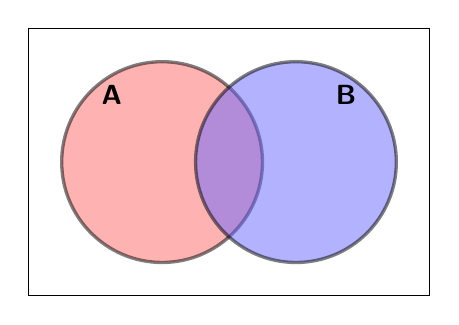
\begin{tikzpicture}[scale=0.85]
\def\circleA{(2,2) circle [radius = 1.5cm]} 
\def\circleB{(4,2) circle [radius = 1.5cm]} 
\draw (0,0) rectangle (6,4);
\draw[very thick, fill=red!60, opacity = 0.5] \circleA;
\node at (1.25,3) {\textbf{A}};
\draw[very thick, fill=blue!60, opacity = 0.5] \circleB;
\node at (4.75,3) {\textbf{B}};
\end{tikzpicture}
\end{center}

\vspace{1in}

\[P(A \text{ or } B) = P(A) + P(B) - P(A \text{ and } B)\]

\vspace{0.25in}

Venn Diagram of Example \ref{tbl_ex}\ref{gen_add}:

\vspace{1in}

\begin{example}
A card is drawn at random from a standard deck of cards. Find each probability.
\begin{enumerate}[(a)]
    \item Selecting a 3 or a club   \vfill 
    \item Drawing a face card or a red card \vfill 
\end{enumerate}
\end{example}

\subsection*{Complement Rule}

\begin{tcolorbox}[colframe=green!20!black, colback = green!30!white,title=\textbf{Complements}]
The \textbf{complement} of an event is the probability the event does \emph{not} happen.
\end{tcolorbox}

\vspace{0.25in}

Event: $P(A)$ \newline\\ 
Complement: $P(A')$

\vspace{0.5in}
\newpage 

\subsection*{``At Least One" Probabilities}

\begin{center}
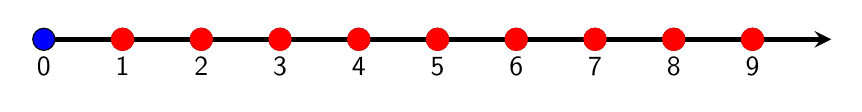
\begin{tikzpicture}
\draw[ultra thick, ->, >=stealth] (0,0) -- (10,0);
\foreach \x in {0,1,...,9}
\draw [fill=blue] (\x,0) circle [radius = 4pt] node [below, yshift=-0.1cm] {$\x$};
\foreach \x in {1,2,...,9}
\draw[color=red,fill=red] (\x,0) circle [radius = 4pt];
\end{tikzpicture}
\end{center}
\begin{itemize}
    \item \emph{At least one} means 1 or 2 or 3 or 4 or ... \newline\\
    \item The complement of \emph{at least one} is {\color{blue}\textbf{none}}.	\newline\\
    \item In general, the complement of \emph{at least n events} is \textbf{\color{red}{$\pmb{n-1}$ events or less.}}
\end{itemize}

\vfill 

\begin{example}
Two dice are rolled. What is the probability of rolling a sum of at least 4?
\begin{center}
\begin{tabular}{c|cccccc}
			&	\textbf{1} & \textbf{2} & \textbf{3} & \textbf{4} & \textbf{5} & \textbf{6} \\ \hline
\textbf{1}	& 2 & 3 & 4 & 5 & 6 & 7 \\
\textbf{2}	& 3 & 4 & 5 & 6 & 7 & 8 \\
\textbf{3}	& 4 & 5 & 6 & 7 & 8 & 9 \\
\textbf{4}	& 5 & 6 & 7 & 8 & 9 & 10 \\
\textbf{5}	& 6 & 7 & 8 & 9 & 10 & 11 \\
\textbf{6}	& 7 & 8 & 9 & 10 & 11 & 12
\end{tabular}
\end{center}
\end{example}

\vfill 

\begin{example}
A certain blood test can determine the presence of a bloodborne pathogen 97\% of the time. If 4 people with the pathogen are given the test, find the probability that the test is accurate for at least one of them.	
\end{example}

\vfill 
\newpage 

\subsection*{Odds}

For events $A$ and $A'$:	\newline\\

\begin{tcolorbox}[colframe=green!20!black, colback = green!30!white,title=\textbf{Odds in Favor}]
The \textbf{odds in favor} of event $A$ to happen are $\frac{A}{A'}$, or $A$ : $A'$
\end{tcolorbox}
\vspace{1in}

\begin{tcolorbox}[colframe=green!20!black, colback = green!30!white,title=\textbf{Odds Against}]
The \textbf{odds against} event $A$ to happen are $\frac{A'}{A}$, or $A'$ : $A$
\end{tcolorbox}	
\vspace{0.25in}
\emph{Note}: Typically when odds are listed, they are the odds against.

\vfill 

\begin{example}
The probability that the Cleveland Browns win the Super Bowl this year is 20\%. What are the odds for and against this?
\end{example}

\vfill 

\begin{example}
A jar contains red and yellow marbles. The odds against selecting a red marble are 5 to 3. What is the probability of selecting a red marble?
\end{example}

\vfill 

\end{document}
